% Options for packages loaded elsewhere
\PassOptionsToPackage{unicode}{hyperref}
\PassOptionsToPackage{hyphens}{url}
%
\documentclass[
]{book}
\usepackage{amsmath,amssymb}
\usepackage{lmodern}
\usepackage{iftex}
\ifPDFTeX
  \usepackage[T1]{fontenc}
  \usepackage[utf8]{inputenc}
  \usepackage{textcomp} % provide euro and other symbols
\else % if luatex or xetex
  \usepackage{unicode-math}
  \defaultfontfeatures{Scale=MatchLowercase}
  \defaultfontfeatures[\rmfamily]{Ligatures=TeX,Scale=1}
\fi
% Use upquote if available, for straight quotes in verbatim environments
\IfFileExists{upquote.sty}{\usepackage{upquote}}{}
\IfFileExists{microtype.sty}{% use microtype if available
  \usepackage[]{microtype}
  \UseMicrotypeSet[protrusion]{basicmath} % disable protrusion for tt fonts
}{}
\makeatletter
\@ifundefined{KOMAClassName}{% if non-KOMA class
  \IfFileExists{parskip.sty}{%
    \usepackage{parskip}
  }{% else
    \setlength{\parindent}{0pt}
    \setlength{\parskip}{6pt plus 2pt minus 1pt}}
}{% if KOMA class
  \KOMAoptions{parskip=half}}
\makeatother
\usepackage{xcolor}
\usepackage{longtable,booktabs,array}
\usepackage{calc} % for calculating minipage widths
% Correct order of tables after \paragraph or \subparagraph
\usepackage{etoolbox}
\makeatletter
\patchcmd\longtable{\par}{\if@noskipsec\mbox{}\fi\par}{}{}
\makeatother
% Allow footnotes in longtable head/foot
\IfFileExists{footnotehyper.sty}{\usepackage{footnotehyper}}{\usepackage{footnote}}
\makesavenoteenv{longtable}
\usepackage{graphicx}
\makeatletter
\def\maxwidth{\ifdim\Gin@nat@width>\linewidth\linewidth\else\Gin@nat@width\fi}
\def\maxheight{\ifdim\Gin@nat@height>\textheight\textheight\else\Gin@nat@height\fi}
\makeatother
% Scale images if necessary, so that they will not overflow the page
% margins by default, and it is still possible to overwrite the defaults
% using explicit options in \includegraphics[width, height, ...]{}
\setkeys{Gin}{width=\maxwidth,height=\maxheight,keepaspectratio}
% Set default figure placement to htbp
\makeatletter
\def\fps@figure{htbp}
\makeatother
\setlength{\emergencystretch}{3em} % prevent overfull lines
\providecommand{\tightlist}{%
  \setlength{\itemsep}{0pt}\setlength{\parskip}{0pt}}
\setcounter{secnumdepth}{5}
\usepackage{ctex}

%\usepackage{xltxtra} % XeLaTeX的一些额外符号
% 设置中文字体
%\setCJKmainfont[BoldFont={黑体},ItalicFont={楷体}]{新宋体}

% 设置边距
\usepackage{geometry}
\geometry{%
	left=2.0cm, right=2.0cm, top=3.5cm, bottom=2.5cm} 

\usepackage{amsthm,mathrsfs}
\usepackage{booktabs}
\usepackage{longtable}
\makeatletter
\def\thm@space@setup{%
	\thm@preskip=8pt plus 2pt minus 4pt
	\thm@postskip=\thm@preskip
}
\makeatother
\ifLuaTeX
  \usepackage{selnolig}  % disable illegal ligatures
\fi
\usepackage[style=apa,]{biblatex}
\IfFileExists{bookmark.sty}{\usepackage{bookmark}}{\usepackage{hyperref}}
\IfFileExists{xurl.sty}{\usepackage{xurl}}{} % add URL line breaks if available
\urlstyle{same} % disable monospaced font for URLs
\hypersetup{
  pdftitle={S416快速入门指南},
  pdfauthor={Leabael},
  hidelinks,
  pdfcreator={LaTeX via pandoc}}

\title{S416快速入门指南}
\author{Leabael}
\date{2022.8.31}

\begin{document}
\maketitle

{
\setcounter{tocdepth}{1}
\tableofcontents
}
\hypertarget{ux7b80ux4ecb}{%
\chapter{简介}\label{ux7b80ux4ecb}}

本指南旨在帮助阅览者快速掌握S416实验室相关仪器操作,学习相关科研技能,培养良好科研习惯。

\hypertarget{instrument}{%
\chapter{实验室主要仪器}\label{instrument}}

\hypertarget{ux4eeaux5668ux5217ux8868}{%
\section{仪器列表}\label{ux4eeaux5668ux5217ux8868}}

\begin{longtable}[]{@{}
  >{\raggedright\arraybackslash}p{(\columnwidth - 4\tabcolsep) * \real{0.3143}}
  >{\raggedright\arraybackslash}p{(\columnwidth - 4\tabcolsep) * \real{0.2286}}
  >{\raggedright\arraybackslash}p{(\columnwidth - 4\tabcolsep) * \real{0.4571}}@{}}
\toprule()
\endhead
仪器名称 & 仪器型号 & 生产厂商 \\
电子天平 & FA214E & 常州市幸运电子设备有限公司 \\
手提式压力蒸汽灭菌器 & XFS-280 & 浙江新丰医疗器械有限公司 \\
电热鼓风干燥箱 & XMA-2000 & 上海秋佐科学仪器有限公司 \\
制冷水浴恒温振荡器 & SHA-2 & 江苏金怡仪器科技有限公司 \\
恒温水浴锅 & HH-S & 江苏省金坛市正基仪器有限公司 \\
超净工作台 & SW-CJ-2D & 上海力辰邦西仪器科技有限公司 \\
高速台式离心机 & TG16-WS & 湖南湘仪实验室仪器开发有限公司 \\
可见分光光度计 & 721 & 上海悦丰仪器仪表有限公司 \\
流式细胞仪 & NovoCyte 2040R & Agilent Technologies \\
紫外仪 & WD-9403C & 北京六一生物科技有限公司 \\
酶标仪 & Multiskan FC & 赛默飞世尔(上海)仪器有限公司 \\
蠕动泵 & BT-200J/YZ1515X & 保定兰格恒流泵有限公司 \\
生化培养箱 & LRH-250 & 上海一恒科学仪器有限公司 \\
& & \\
& & \\
\bottomrule()
\end{longtable}

\hypertarget{ux8d85ux51c0ux5de5ux4f5cux53f0}{%
\section{超净工作台}\label{ux8d85ux51c0ux5de5ux4f5cux53f0}}

\textbf{用前准备}

\begin{enumerate}
\def\labelenumi{\arabic{enumi}.}
\tightlist
\item
  穿戴好实验服,佩戴好手套
\item
  检查超净工作台设备情况,在设备良好的情况下继续使用
\end{enumerate}

\begin{figure}

{\centering 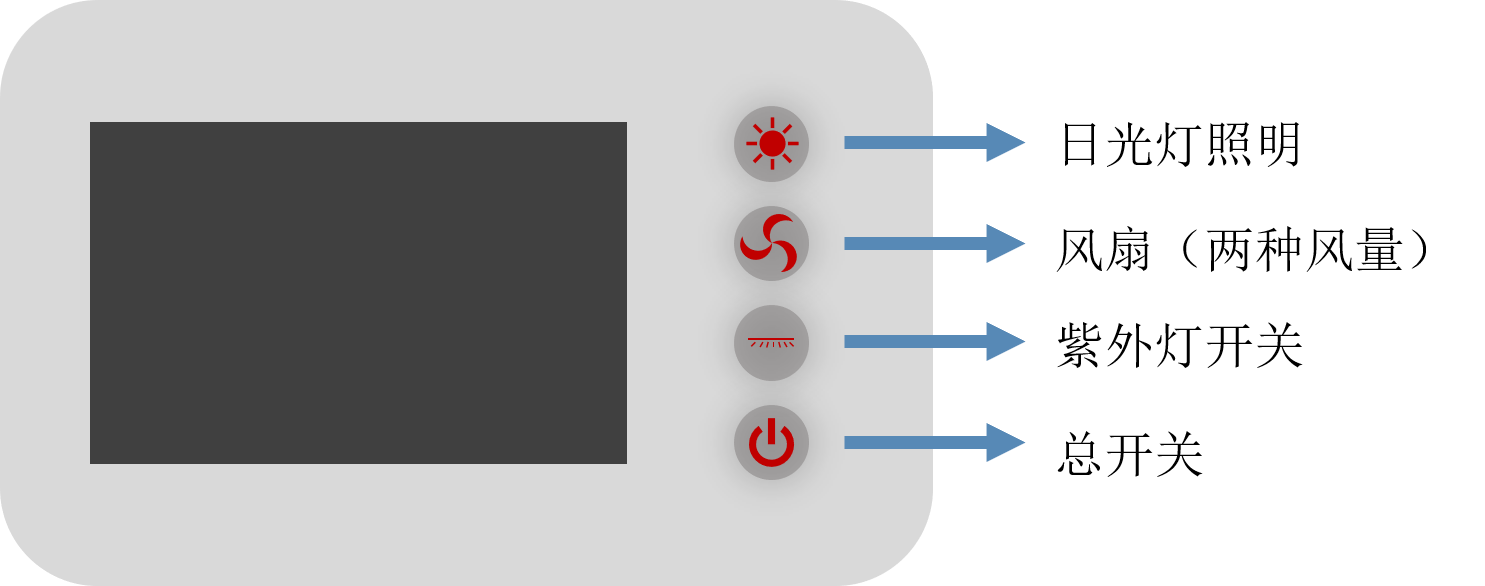
\includegraphics[width=0.5\linewidth]{images/超净工作台} 

}

\caption{超净工作台}\label{fig:unnamed-chunk-1}
\end{figure}

\textbf{操作步骤}

\begin{enumerate}
\def\labelenumi{\arabic{enumi}.}
\tightlist
\item
  使用前30分钟放入实验所需用品,打开紫外灯,照射20分钟后打开风扇,对操作区域进行灭菌
\item
  打开日光灯(会自动关闭紫外灯)和风扇进行实验操作
\item
  操作过程中拿取物品,需要物品和双手喷涂酒精后进入超净工作台
\item
  操作结束后整理工作台面,喷洒75\%乙醇溶液,并用餐巾纸由内到外擦拭干净,打开紫外灯照射15分钟,结束使用
\end{enumerate}

\textbf{注意事项}

\begin{enumerate}
\def\labelenumi{\arabic{enumi}.}
\tightlist
\item
  实验操作过程中禁止打开紫外灯
\item
  操作过程遇到飞虫进入,立即停止操作,在没有实验用菌的情况下进行紫外消杀
\item
  紫外灯不可长时间(\textless45min)开启
\item
  接触电器开关保持手部干燥
\item
  保持工作台内干燥和清洁
\item
  他人使用超净台时,尽可能减少超净台附近的走动
\item
  尽可能减少手部饰品、手表的佩戴
\end{enumerate}

\textbf{操作技巧}

\begin{enumerate}
\def\labelenumi{\arabic{enumi}.}
\tightlist
\item
  实验操作复杂可提前将打印好的操作步骤黏贴于超净台控制面板下方区域
\item
  操作过程中人为将台面分为污染高、低风险区(按照个人操作习惯)

  \begin{itemize}
  \tightlist
  \item
    高风险区:放置废液缸、取样菌种、比色皿(调节OD值)、含有样品的培养皿等
  \item
    低风险区:移液枪、涂布棒、平板、未加菌的培养体系、枪头等
  \end{itemize}
\item
  所有离心管和玻璃瓶在使用完成后对敞口进行密封
\end{enumerate}

\textbf{仪器维护}

\begin{enumerate}
\def\labelenumi{\arabic{enumi}.}
\tightlist
\item
  定期检查紫外灯管发光处氧化情况
\item
  定期擦拭超净台隔断玻璃内外面
\item
  定期检查超净台隔断玻璃密封条状态
\end{enumerate}

\textbf{参考资料}

\begin{enumerate}
\def\labelenumi{\arabic{enumi}.}
\tightlist
\item
  \href{https://www.bilibili.com/video/BV1H64y1S7JC}{超净工作台内部操作}
\item
  \href{https://www.bilibili.com/video/BV1L44y1r7wf}{超净工作台使用说明}
\end{enumerate}

\hypertarget{ux79bbux5fc3ux673a}{%
\section{离心机}\label{ux79bbux5fc3ux673a}}

\textbf{用前准备}

\begin{enumerate}
\def\labelenumi{\arabic{enumi}.}
\tightlist
\item
  打开电源开关,确定显示编号与转头相符
\item
  检查转头无异常碰擦声响,过大振动和噪音;若存在异常立即停止使用,排除故障后继续使用
\end{enumerate}

\textbf{操作步骤}

\begin{enumerate}
\def\labelenumi{\arabic{enumi}.}
\tightlist
\item
  设定所需转速和离心时间,并再次检查转头编号和显示数字是否一致
\item
  将离心管管壁擦拭干净中心对称或轴对称放入离心机内,如样品数量不够需要配平
\item
  旋盖离心管需要检查管盖是否拧紧,高速离心管需要盖紧后加盖转头盖
\item
  开始离心,离心过程中不得随意离开,应随时观察离心机上的仪表是否正常工作,如有异常的声音应立即停机检查,及时排除故障
\item
  在离心机完全停止后方可开盖拿取离心样品
\item
  检查离心机转头,及时清洗、擦干,关闭电源
\end{enumerate}

\textbf{注意事项}

\begin{enumerate}
\def\labelenumi{\arabic{enumi}.}
\tightlist
\item
  转头是离心机中须重点保护的部件,不能碰撞
\item
  低温离心时,转头在使用前应放置于冰箱中进行预冷,离心结束后倒置转头并擦干腔内余水
\item
  开机前必须检查转头和转头盖是否拧紧无缝隙,确认无误后方可启动离心机
\end{enumerate}

\hypertarget{ux5206ux5149ux5149ux5ea6ux8ba1}{%
\section{分光光度计}\label{ux5206ux5149ux5149ux5ea6ux8ba1}}

\textbf{用前准备}

\begin{enumerate}
\def\labelenumi{\arabic{enumi}.}
\tightlist
\item
  取下覆盖塑料,检查仪器状态,保证仪器状态良好后继续使用
\item
  根据样品需要,准备清洁后的石英或玻璃比色皿
\end{enumerate}

\textbf{操作步骤}

\begin{enumerate}
\def\labelenumi{\arabic{enumi}.}
\tightlist
\item
  打开仪器开关,掀开样品室暗箱盖,调节(检查)所需波长,预热30分钟
\item
  将背景校正液用移液枪添加进比色皿\(\dfrac{2}{3}\)处(约3 mL),用纸巾擦清外壁,放入样品室内对准光路,关闭暗箱盖后进行校正
\item
  添加1 mL样品润洗后,将样品添加进比色皿\(\dfrac{2}{3}\)处(约3 mL),用纸巾擦清外壁,放入样品室内对准光路,关闭暗箱盖后进行测量
\item
  待读数稳定后记录数据(在仪器预热充分情况下为提示音响起)
\item
  检查并清理样品室,洗净并晾干比色皿,关闭电源并覆盖塑料保存
\end{enumerate}

\textbf{注意事项}

\begin{enumerate}
\def\labelenumi{\arabic{enumi}.}
\tightlist
\item
  使用本仪器前,使用者应该首先了解本仪器的结构和工作原理,以及各个按钮功能
\item
  拿取比色皿需注意捏毛面,不要用手直接接触光面
\item
  将比色皿放入样品室需注意光面透光
\item
  分光光度计不可长时间开启
\item
  比色皿测样前注意内部气泡是否去除
\end{enumerate}

\hypertarget{ux9ad8ux6e29ux70d8ux7bb1}{%
\section{高温烘箱}\label{ux9ad8ux6e29ux70d8ux7bb1}}

\textbf{用前准备}

\begin{enumerate}
\def\labelenumi{\arabic{enumi}.}
\tightlist
\item
  在断电情况下用酒精擦拭烘箱内部和样品架表面,清理掉落标签,等待酒精充分挥发后关闭箱门通电
\item
  打开排风扇,设定目标温度,等待升温
\item
  观察烘箱运行情况,待稳定后使用
\end{enumerate}

操作步骤

\begin{enumerate}
\def\labelenumi{\arabic{enumi}.}
\tightlist
\item
  取样时缓慢打开箱门,切勿在高温状态下快速或急速开启箱门
\item
  放置物品时,上下四周应留存一定空间,保持箱内气流畅通
\item
  烘箱上层放置灭菌后枪头盒和干净的玻璃瓶盖;中层放置灭菌后培养液、离心管、滤膜等;下层放置灭菌后培养基和备用玻璃瓶
\item
  将箱门轻轻关闭,且需检查箱门与硅胶密封条紧密结合
\end{enumerate}

\textbf{注意事项}

\begin{enumerate}
\def\labelenumi{\arabic{enumi}.}
\tightlist
\item
  含易燃易爆等有机挥发性溶剂或助剂禁止放入箱内
\item
  关闭时不可太用力,避免造成箱体大幅振动
\item
  戴隔热手套取样
\item
  拿取物品时避免头部直接正对箱门开口,需待箱内热量散失5-10秒
\item
  废弃物品不可随手弃置于烘箱周围
\end{enumerate}

\hypertarget{ux9ad8ux538bux706dux83ccux9505}{%
\section{高压灭菌锅}\label{ux9ad8ux538bux706dux83ccux9505}}

\textbf{用前准备}

\begin{enumerate}
\def\labelenumi{\arabic{enumi}.}
\tightlist
\item
  穿戴好实验服,戴好隔热手套
\item
  检查灭菌锅水位(内筒边缘与外筒持平或略高,灭菌物品放入后内筒仍有浮力)
\item
  检查锅盖排气阀、安全阀状态
\item
  检查灭菌压力设置
\end{enumerate}

\textbf{操作步骤}

\begin{enumerate}
\def\labelenumi{\arabic{enumi}.}
\tightlist
\item
  将需灭菌的物品放入灭菌锅内,不可过多放置

  \begin{itemize}
  \tightlist
  \item
    玻璃瓶类:培养液、培养基、缓冲液、无菌水等需要摇匀后略松瓶盖
  \item
    离心管类:5 mL及以下离心管装入烧杯后用锡箔纸封闭杯口后放入,5 mL及以上离心管需要管盖分离灭菌(防止内外压力过大使离心管变形)
  \item
    枪头类:装填完成后密封放入
  \end{itemize}
\item
  打开电源,设置温度后(一般不需操作,但需检查),转动时间开关(预热),排出内筒冷空气
\item
  关紧锅盖(压力表导管放入内筒检测口中,压住锅盖,依次拧紧螺丝),检查排气阀、安全阀状态(关排气阀,检查安全阀是否保持关合状态)
\item
  菌锅开始工作(待温度升至105 °C,检查灭菌锅是否漏气;温度至121 °C时,重新设置时间为40 min)
\item
  设定时间结束,关闭电源,待压力表指针降至最低时,打开放气阀缓慢放气
\item
  放气阀无蒸汽排除时,方可开启锅盖
\item
  将锅内物品取出放入烘箱或室温冷却(装有试剂的玻璃瓶盖需要拧紧,未装有试剂的玻璃瓶需要取下瓶盖)
\item
  拔下插头
\end{enumerate}

\textbf{注意事项}

\begin{enumerate}
\def\labelenumi{\arabic{enumi}.}
\tightlist
\item
  第一次使用必须有人在旁指导
\item
  气未放尽前,不得开启高压锅
\item
  灭菌物品应符合高压灭菌要求
\item
  切忌将培养基封闭在锅内时间过长
\item
  放进去的瓶子表面都不要有污垢,长期积累会堵塞灭菌锅
\item
  操作过程,小心烫伤
\item
  内筒内不能有积液
\item
  备用玻璃瓶应用纯水/超纯水冲洗干净后放入
\item
  灭菌液体不得超过所装玻璃瓶的刻度容积
\end{enumerate}

\textbf{仪器维护}

\begin{enumerate}
\def\labelenumi{\arabic{enumi}.}
\tightlist
\item
  定期清理内筒
\item
  定期检查压力设置
\item
  定期检查安全阀和排气阀情况
\end{enumerate}

\textbf{应急预案}

\begin{enumerate}
\def\labelenumi{\arabic{enumi}.}
\tightlist
\item
  仪器异常时先检查压力表(温度或压力在红色区域)指示,如超过允许最大压力而安全调没有跳起,应立即切断电源并将排气阀旋到最大
\item
  如压力表指示在红色区域,应观察温度设置是否正确
\item
  如遇其他问题必须通知专业维修人员进行检修
\end{enumerate}

\hypertarget{ux6052ux6e29ux6c34ux6d74ux6447ux5e8a}{%
\section{恒温水浴摇床}\label{ux6052ux6e29ux6c34ux6d74ux6447ux5e8a}}

用前准备

\begin{enumerate}
\def\labelenumi{\arabic{enumi}.}
\tightlist
\item
  本仪器使用电源为220V交流电,使用前请确定电源插座额定电流不小于10A,并具有安全接地装置,否则请更换插座
\item
  在使用该仪器之前,如有实验液体撒入箱体内,应及时擦洗干净以免腐蚀仪器
\item
  检查振荡器内用水状况
\end{enumerate}

\textbf{操作步骤}

\begin{enumerate}
\def\labelenumi{\arabic{enumi}.}
\tightlist
\item
  设定摇晃速度,培养温度,确保振荡器内水位高度(一般高于震荡台)
\item
  将所需震荡物品密封后平稳放置在暂停摇晃的震荡台上(倾斜可能导致甩出)
\item
  打开开关,开始摇晃培养
\end{enumerate}

\textbf{注意事项}

\begin{enumerate}
\def\labelenumi{\arabic{enumi}.}
\tightlist
\item
  当仪器托盘做振荡时,请勿将手伸入工作室内接触正在振荡的托盘或烧瓶
\item
  在使用振荡功能时,以防烧瓶甩出,应在振荡器停止的状态下,才能打开仪器门。在放好烧瓶后,关闭好振荡培养箱门后,方可启动振荡功能
\item
  仪器应做好经常性清洁工作(震荡期内水应干净无异味、异物),保持工作台面和操作面板的整洁
\item
  仪器应旋转平稳,不能侧倾使用
\item
  设备在搬运时,倾角不得大于45度
\item
  摇晃溶液不得大于瓶身\(\dfrac{2}{3}\)
\end{enumerate}

\textbf{仪器维护}

\begin{enumerate}
\def\labelenumi{\arabic{enumi}.}
\tightlist
\item
  仪器内水产生异味,伴有异物需取出培养样品,全面清洁摇床内部

  \begin{itemize}
  \tightlist
  \item
    倒净摇床内部用水,拆下摇床
  \item
    用刷子彻底清洁摇床和基座内部
  \item
    用配置好的84溶液浸泡洗净的摇床和基座内部30分钟,冲洗干净
  \item
    组装并重新添加水浴用水
  \end{itemize}
\end{enumerate}

\hypertarget{ux4f4eux6e29ux51b0ux67dc}{%
\section{低温冰柜}\label{ux4f4eux6e29ux51b0ux67dc}}

\textbf{用前准备}

\begin{enumerate}
\def\labelenumi{\arabic{enumi}.}
\tightlist
\item
  佩戴防低温手套
\item
  检查冰柜温度情况
\end{enumerate}

\textbf{操作步骤}

\begin{enumerate}
\def\labelenumi{\arabic{enumi}.}
\tightlist
\item
  打开冰柜柜门后提取所需离心管盒存放架
\item
  拿取需要的样品,并放回离心管盒存放架
\item
  关闭冰柜门,确保密封
\end{enumerate}

\textbf{注意事项}

\begin{enumerate}
\def\labelenumi{\arabic{enumi}.}
\tightlist
\item
  冰柜柜门上不得放置任何物品
\item
  小心冻伤
\end{enumerate}

\hypertarget{ux6052ux6e29ux57f9ux517bux7bb1}{%
\section{恒温培养箱}\label{ux6052ux6e29ux57f9ux517bux7bb1}}

\textbf{操作步骤}

\begin{enumerate}
\def\labelenumi{\arabic{enumi}.}
\tightlist
\item
  设定培养温度
\item
  打开箱门,放入密封、标记好的样品
\item
  关闭并密封箱门
\end{enumerate}

\textbf{注意事项}

\begin{enumerate}
\def\labelenumi{\arabic{enumi}.}
\tightlist
\item
  箱壁内胆和设备表面要经常擦拭,以保持清洁
\item
  把需作培养实验的物品放入培养箱工作室内,上、下四周应留存一定空间保持工作室内气流畅通,关好箱门
\end{enumerate}

\hypertarget{ux9176ux6807ux4eea}{%
\section{酶标仪}\label{ux9176ux6807ux4eea}}

\textbf{操作步骤}

\begin{enumerate}
\def\labelenumi{\arabic{enumi}.}
\tightlist
\item
  打开电源,设定好测量数据,放入96孔板
\item
  测量完成后对数据进行拍照记录,取出96孔板并确保仪器清洁
\item
  关闭电源并收纳
\end{enumerate}

\textbf{参考资料}

\begin{enumerate}
\def\labelenumi{\arabic{enumi}.}
\tightlist
\item
  \href{https://www.bilibili.com/video/BV1i5411A7pp}{酶标仪操作全流程}
\end{enumerate}

\hypertarget{ux79fbux6db2ux67aaux52a9ux5438ux5668}{%
\section{移液枪\&助吸器}\label{ux79fbux6db2ux67aaux52a9ux5438ux5668}}

\hypertarget{ux79fbux6db2ux67aa}{%
\subsection{移液枪}\label{ux79fbux6db2ux67aa}}

\textbf{用前准备}

\begin{enumerate}
\def\labelenumi{\arabic{enumi}.}
\tightlist
\item
  检查移液枪各部分完整度,确保套筒口(11)洁净
\end{enumerate}

\begin{figure}

{\centering 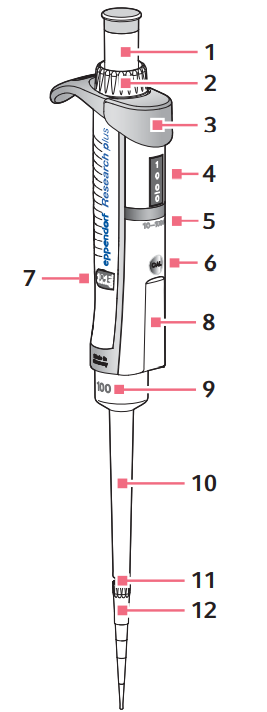
\includegraphics[width=0.25\linewidth]{images/Pasted image 20220803010953} 

}

\caption{移液枪结构图}\label{fig:unnamed-chunk-2}
\end{figure}

\textbf{操作步骤}

\begin{enumerate}
\def\labelenumi{\arabic{enumi}.}
\tightlist
\item
  调节操作容量

  \begin{itemize}
  \tightlist
  \item
    顺时针调低容量,一步到位直接使用
  \item
    逆时针调高容量,应先调至超过设定体积刻度,再回调至设定体积,保证移液器的精确度
  \end{itemize}
\item
  枪头装卸

  \begin{itemize}
  \tightlist
  \item
    选用对应量程匹配的枪头
  \item
    竖直嵌入并左右旋转拧紧枪头
  \item
    严禁竖直敲打牢固枪头
  \end{itemize}
\end{enumerate}

\begin{center}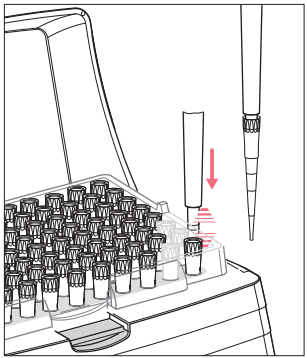
\includegraphics[width=0.3\linewidth]{images/Pasted image 20220803013705} \end{center}

\begin{enumerate}
\def\labelenumi{\arabic{enumi}.}
\setcounter{enumi}{2}
\tightlist
\item
  吸液及放液

  \begin{itemize}
  \item
    吸液

    \begin{itemize}
    \item
      按照吸取液体体积,确定枪头浸没深度
    \item
      在转移液体前应润洗1-3次

      \textbf{正向吸液}(适用于流动性较好,粘度较低液体)

      \begin{itemize}
      \item
        按下配药按钮到第一阶段
      \item
        将移液管尖端垂直浸入液体
      \item
        保持浸没深度,缓慢回弹配药按钮,等待液体被吸取 如有必要将枪头尖端多余液体挂回离心管壁
      \item
        将移液管尖端以陡峭角度放在离心管壁上
      \item
        慢慢按下配药按钮至第一阶段,充分排出液体后按至第二阶段
      \item
        按住分配按钮将枪头尖端多余液体挂回离心管壁,缓慢回弹分配按钮

        \textbf{反向吸液}(适用于粘度较高,易起泡液体)
      \item
        按下配药按钮到第二阶段
      \item
        将移液管尖端垂直浸入液体
      \item
        保持浸没深度,缓慢回弹配药按钮,等待液体被吸取 如有必要将枪头尖端多余液体挂回离心管壁
      \item
        将移液管尖端以陡峭角度放在离心管壁上
      \item
        慢慢按下配药按钮至第一阶段
      \item
        按住分配按钮将枪头尖端多余液体挂回离心管壁,缓慢回弹分配按钮
      \item
        丢弃多余液体
      \end{itemize}
    \end{itemize}
  \end{itemize}
\end{enumerate}

\begin{figure}

{\centering 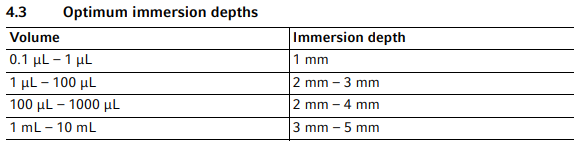
\includegraphics[width=0.5\linewidth]{images/Pasted image 20220802014111} 

}

\caption{吸液深度最佳示意表}\label{fig:unnamed-chunk-4}
\end{figure}

\textbf{注意事项}

\begin{enumerate}
\def\labelenumi{\arabic{enumi}.}
\tightlist
\item
  使用完成后务必将量程调到最大
\item
  使用前后均需消毒表面
\item
  使用后应放置在移液枪架上
\item
  当移液器枪头里有液体时,切勿将移液器水平放置或倒置,以免液体倒流腐蚀活塞弹簧
\item
  分配按钮需要缓慢操作,放置速度过快,液体冲入移液枪内部
\item
  提前熟悉各移液枪适配枪头的最大量程(一些枪头不能达到移液枪最大量程),尤其在进行反向吸液操作时需要注意量程
\end{enumerate}

\textbf{仪器维护}

\begin{enumerate}
\def\labelenumi{\arabic{enumi}.}
\tightlist
\item
  \href{https://www.bilibili.com/video/BV1FT4y1o7iy}{Eppendorf手动移液器维护保养}
\item
  \href{https://www.bilibili.com/video/BV1UZ4y1z7oZ}{大龙移液枪的日常维护与校准}
\end{enumerate}

\textbf{参考资料}

\begin{enumerate}
\def\labelenumi{\arabic{enumi}.}
\tightlist
\item
  \href{https://www.eppendorf.com/fileadmin/knowledgebase/asset/CN-zh/186591.pdf}{移液枪使用手册}
\item
  \href{https://www.bilibili.com/video/BV17b4y1J7mN}{移液枪量程设置}
\item
  \href{https://www.bilibili.com/video/BV1iZ4y1f7sq}{移液枪枪头润洗}
\item
  \href{https://www.bilibili.com/video/BV1XS4y1j7Uk}{移液枪浸入深度和吸液角度}
\item
  \href{https://www.bilibili.com/video/BV1eY411h7V5}{移液枪吸液操作}
\item
  \href{https://www.bilibili.com/video/BV1ES4y1f7uA}{移液枪分液操作}
\item
  \href{https://www.bilibili.com/video/BV15b4y1J7RF}{移液操作循环}
\item
  \href{https://www.bilibili.com/video/BV17e4y1d7ex}{移液枪正反向移液}
\item
  \href{https://www.bilibili.com/video/BV1g3411g7ZY}{涡旋振荡器和移液枪-溶液混匀}
\item
  \href{https://www.bilibili.com/video/BV1Av4y1G7r4}{正确使用移液枪}
\end{enumerate}

\hypertarget{ux52a9ux5438ux5668}{%
\subsection{助吸器}\label{ux52a9ux5438ux5668}}

\textbf{参考资料}

\begin{enumerate}
\def\labelenumi{\arabic{enumi}.}
\tightlist
\item
  \href{http://www.sccos.cn/9.pdf}{电动助吸器快速操作指南}
\item
  \href{https://www.eppendorf.com/product-media/doc/en/166659_Short-Instructions/Eppendorf_Liquid-Handling_Short-instructions_Easypet-3_Easypet-3.pdf?_ga=2.144546805.1938597545.1659465477-672298651.1659375433}{电动助吸器官方快速操作指南}
\item
  \href{https://www.eppendorf.com/product-media/doc/zh/166652_Operating-Manual/Eppendorf_Liquid-Handling_Operating-manual_Easypet-3_Easypet-3.pdf?_ga=2.115859398.1938597545.1659465477-672298651.1659375433}{Eppendorf Liquid-Handling Operating-manual}
\end{enumerate}

\hypertarget{ux7535ux5b50ux5929ux5e73}{%
\section{电子天平}\label{ux7535ux5b50ux5929ux5e73}}

\textbf{用前准备}

\begin{enumerate}
\def\labelenumi{\arabic{enumi}.}
\tightlist
\item
  检查天平的水平状态
\item
  检查天平洁净程度
\end{enumerate}

\textbf{操作步骤}

\begin{enumerate}
\def\labelenumi{\arabic{enumi}.}
\tightlist
\item
  打开开关预热(30 min - 1 h)
\item
  设定称量单位,沿对角线对折称量纸,放入称量纸后封闭去皮,逐渐加入待称物质,直到所需重量为止
\item
  关闭侧门待示数稳定
\item
  称量结束应及时除去称量瓶(纸),关上侧门,并做好使用情况登记
\item
  将防尘塑料罩上,切断电源
\end{enumerate}

\textbf{注意事项}

\begin{enumerate}
\def\labelenumi{\arabic{enumi}.}
\tightlist
\item
  天平应放置在牢固平稳水泥台或木台上,室内要求清洁、干燥及较恒定的温度,同时应避免光线直接照射到天平上
\item
  称量时应从侧门取放物质,读数时应关闭箱门以免空气流动引起天平摆动。前门仅在检修或清除残留物质时使用
\item
  电子精密天平若长时间不使用,则应定时通电预热,每周一次,每次预热2h,以确保仪器始终处于良好使用状态
\item
  挥发性、腐蚀性、强酸强碱类物质应盛于带盖称量瓶内称量,防止腐蚀天平
\item
  时刻保持操作面清洁,如有药品残留,应立即用毛刷出去表面污物
\item
  不能超载,称重不能超过最大称量量程
\item
  电子分析天平使用一定时间后,要送计量检定单位进行校验和调修
\item
  最少半年对电子分析天平进行一次全方位的清理作业
\end{enumerate}

\hypertarget{ux6d41ux5f0fux7ec6ux80deux4eea}{%
\section{流式细胞仪}\label{ux6d41ux5f0fux7ec6ux80deux4eea}}

\textbf{用前准备}

\begin{enumerate}
\def\labelenumi{\arabic{enumi}.}
\tightlist
\item
  检查仪器储液装置waste(红色)和鞘液(绿色),正常情况下在开机后储液装置指示灯为绿色
\end{enumerate}

\begin{figure}

{\centering 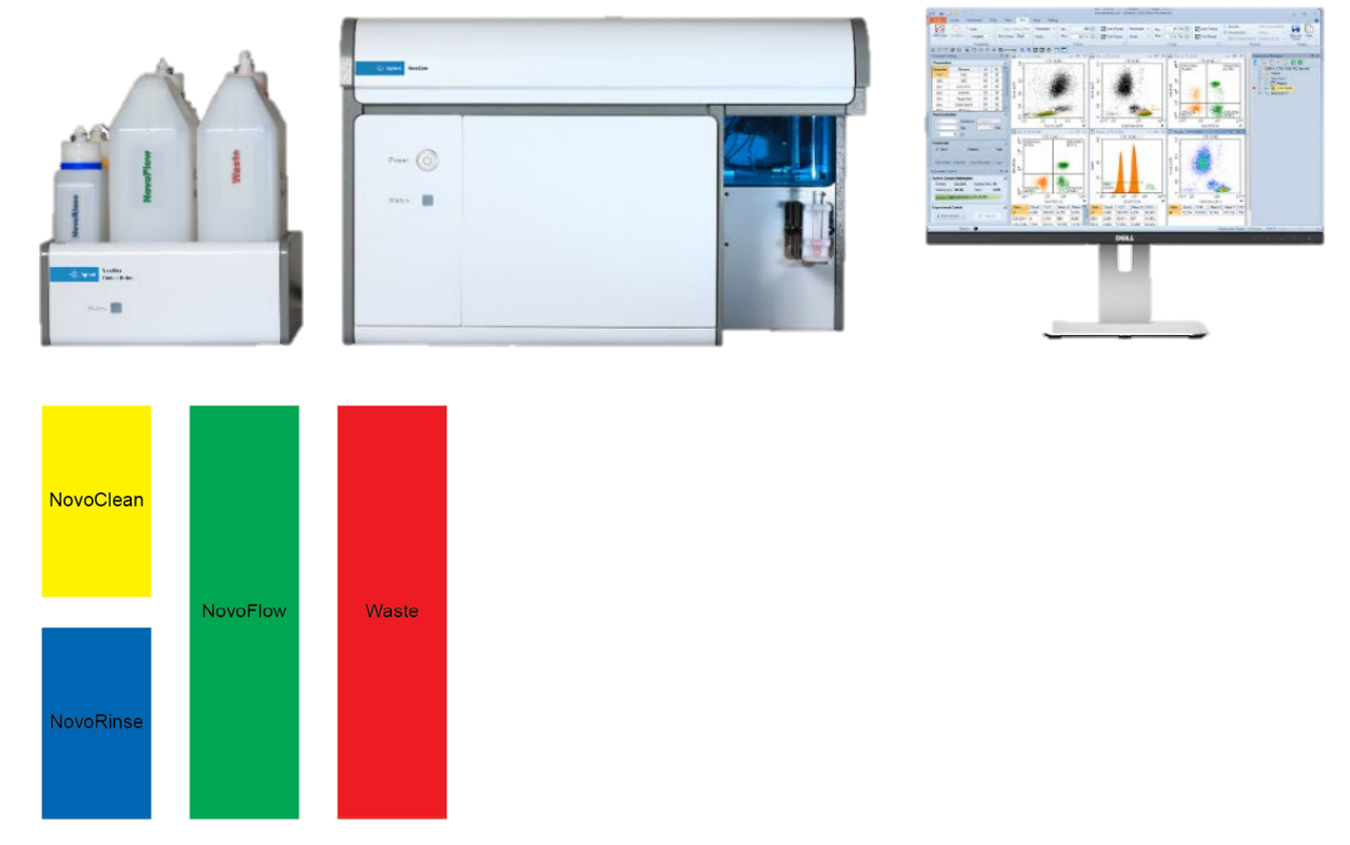
\includegraphics[width=0.5\linewidth]{images/流式细胞仪} 

}

\caption{吸液深度最佳示意表}\label{fig:unnamed-chunk-5}
\end{figure}

\textbf{操作步骤}

\begin{enumerate}
\def\labelenumi{\arabic{enumi}.}
\tightlist
\item
  打开仪器和显示器开关
\item
  第一次使用新建自己的工作文件夹用于存储数据,打开测量软件存储在个人工作文件夹
\item
  新建样本组和样本,进行命名后设置各样本测量界面参数
\item
  测样
\item
  导出检测报告并拷贝
\item
  关机
\end{enumerate}

\textbf{注意事项}

\begin{enumerate}
\def\labelenumi{\arabic{enumi}.}
\tightlist
\item
  必须观摩至少一次后方可上机操作,且第一次操作必须有熟练掌握的人员在旁指导
\item
  每个实验组测样后需要冲洗取样针
\item
  测样时需要对准离心管管口,静止撞针
\item
  仪器本身和储液装置指示灯为绿色方可进行实验
\end{enumerate}

\textbf{参考资料}

\begin{enumerate}
\def\labelenumi{\arabic{enumi}.}
\tightlist
\item
  \href{https://www.agilent.com.cn/cs/library/usermanuals/public/150014-NovoCyte\%20Flow\%20Cytometer\%20Operator\textquotesingle{}s\%20Guide\%20(RUO).pdf}{150014-NovoCyte Flow Cytometer Operator's Guide}
\end{enumerate}

\hypertarget{materials}{%
\chapter{试剂、菌株}\label{materials}}

\hypertarget{ux4e3bux8981ux8bd5ux5242}{%
\section{主要试剂}\label{ux4e3bux8981ux8bd5ux5242}}

\begin{longtable}[]{@{}
  >{\raggedright\arraybackslash}p{(\columnwidth - 8\tabcolsep) * \real{0.2500}}
  >{\raggedright\arraybackslash}p{(\columnwidth - 8\tabcolsep) * \real{0.1618}}
  >{\raggedright\arraybackslash}p{(\columnwidth - 8\tabcolsep) * \real{0.2206}}
  >{\raggedright\arraybackslash}p{(\columnwidth - 8\tabcolsep) * \real{0.2206}}
  >{\raggedright\arraybackslash}p{(\columnwidth - 8\tabcolsep) * \real{0.1471}}@{}}
\toprule()
\begin{minipage}[b]{\linewidth}\raggedright
试剂名称
\end{minipage} & \begin{minipage}[b]{\linewidth}\raggedright
保存方法
\end{minipage} & \begin{minipage}[b]{\linewidth}\raggedright
浓度/纯度
\end{minipage} & \begin{minipage}[b]{\linewidth}\raggedright
生产厂家
\end{minipage} & \begin{minipage}[b]{\linewidth}\raggedright
主要用途
\end{minipage} \\
\midrule()
\endhead
LB肉汤 & 室温 & BR & 青岛海博生物技术有限公司 & 培养细菌 \\
Agar琼脂 & 室温 & BR & 北京酷来搏科技有限公司 & 凝固剂 \\
20×PBS磷酸盐缓冲液 & 室温 & BR & 上海源叶生物科技有限公司 & 缓冲溶液 \\
无水乙醇 & 室温 & 消毒 & & \\
甘油 & 室温 & 上海源叶生物科技有限公司 & 细菌防冻 & \\
葡萄糖 & 室温 & Sigma-Aldrich & 微生物营养物 & \\
乙酸钠 & 室温 & Sigma-Aldrich & 微生物营养物 & \\
盐酸四环素 (Tet) & -20 °C & 900 μg/mg & 上海源叶生物科技有限公司 & 抗生素 \\
硫酸链霉素 (Sul) & 2-6 °C & 上海源叶生物科技有限公司 & 抗生素 & \\
卡纳硫酸 (Kan) & 2-6 °C & 上海源叶生物科技有限公司 & 抗生素 & \\
氨苄青霉素 (Amp) & 2-6 °C & 上海源叶生物科技有限公司 & 抗生素 & \\
碘化丙啶PI染色液 & 避光 -20 °C & 1 mg/mL & 北京雷根生物技术有限公司 & 细胞膜通透性测定 \\
2',7'-二氯荧光素二乙酸酯 & 避光 -20 °C & ≥ 97\% & Sigma-Aldrich & 活性氧产量测定 \\
次氯酸钠 & 2-6 °C & 上海源叶生物科技有限公司 & 消毒 & \\
待补充 & & & & \\
待补充 & & & & \\
待补充 & & & & \\
待补充 & & & & \\
待补充 & & & & \\
\bottomrule()
\end{longtable}

\hypertarget{ux4e3bux8981ux83ccux682a}{%
\section{主要菌株}\label{ux4e3bux8981ux83ccux682a}}

\begin{longtable}[]{@{}
  >{\raggedright\arraybackslash}p{(\columnwidth - 6\tabcolsep) * \real{0.6338}}
  >{\raggedright\arraybackslash}p{(\columnwidth - 6\tabcolsep) * \real{0.1549}}
  >{\raggedright\arraybackslash}p{(\columnwidth - 6\tabcolsep) * \real{0.1268}}
  >{\raggedright\arraybackslash}p{(\columnwidth - 6\tabcolsep) * \real{0.0845}}@{}}
\toprule()
\begin{minipage}[b]{\linewidth}\raggedright
名称
\end{minipage} & \begin{minipage}[b]{\linewidth}\raggedright
保存方法
\end{minipage} & \begin{minipage}[b]{\linewidth}\raggedright
主要用途
\end{minipage} & \begin{minipage}[b]{\linewidth}\raggedright
购买厂家
\end{minipage} \\
\midrule()
\endhead
Escherichia coli str. K-12 substr. MG1655 & -20-80°C & 突变 & \\
Escherichia coli HB101 & -20-80°C & 接合转移 & \\
Escherichia coli HB101 with Plasmid RP4 & -20-80°C & 杀菌、接合转移 & \\
Escherichia coli HB101 with Plasmid PWH1266 & -20-80°C & 转化 & \\
\bottomrule()
\end{longtable}

\hypertarget{protocols}{%
\chapter{常用实验操作流程}\label{protocols}}

❗该部分主要介绍S416实验室常用实验的操作流程,具体实验方案仍需根据实际情况自行修改。

\hypertarget{ux5faeux751fux7269ux57f9ux517bux5b9eux9a8c}{%
\section{微生物培养实验}\label{ux5faeux751fux7269ux57f9ux517bux5b9eux9a8c}}

\hypertarget{ux83ccux682aux57f9ux517b}{%
\subsection{菌株培养}\label{ux83ccux682aux57f9ux517b}}

将菌种从冰箱取出解冻,从烘箱里取一个装有50ml或100ml培养液的玻璃瓶冷却到室温。将菌种按1\%比例加入到培养液中,摇匀(超净台操作),过夜培养

\begin{longtable}[]{@{}
  >{\raggedright\arraybackslash}p{(\columnwidth - 6\tabcolsep) * \real{0.5000}}
  >{\raggedright\arraybackslash}p{(\columnwidth - 6\tabcolsep) * \real{0.1556}}
  >{\raggedright\arraybackslash}p{(\columnwidth - 6\tabcolsep) * \real{0.1667}}
  >{\raggedright\arraybackslash}p{(\columnwidth - 6\tabcolsep) * \real{0.1778}}@{}}
\toprule()
\begin{minipage}[b]{\linewidth}\raggedright
\end{minipage} & \begin{minipage}[b]{\linewidth}\raggedright
培养条件
\end{minipage} & \begin{minipage}[b]{\linewidth}\raggedright
抗生素
\end{minipage} & \begin{minipage}[b]{\linewidth}\raggedright
备注
\end{minipage} \\
\midrule()
\endhead
Escherichia coli str. K-12 substr. MG1655 & 37°C, 150rpm & / & \\
Escherichia coli HB101 & 37°C, 150rpm & Sul & 抗生素母液稀释1000倍添加 \\
Escherichia coli K-12 LE392 with Plasmid RP4 & 37°C, 150rpm & Kan, Amp, Tet & 抗生素母液稀释1000倍添加 \\
Escherichia coli HB101 with Plasmid PWH1266 & 37°C, 150rpm & & \\
\bottomrule()
\end{longtable}

\hypertarget{ux83ccux682aux7eafux5316}{%
\subsection{菌株纯化}\label{ux83ccux682aux7eafux5316}}

\begin{enumerate}
\def\labelenumi{\arabic{enumi}.}
\tightlist
\item
  先倒至数个空白板(纯化不含抗性的菌)/抗性板(纯化抗性菌)
\item
  将要纯化的菌隔夜培养/已有菌液则不需培养
\item
  利用划线平板法(用接种环沾取少量菌液),在培养皿上划三条线,在最后一条线的基础上再划三条,重复以上步骤。可做多个板子,封口倒置放入密封袋
\item
  隔夜培养后,用接种环挑选单个菌株放入液体培养液中(做空白对照)
\item
  隔夜培养后用甘油保存
\end{enumerate}

\hypertarget{ux83ccux682aux4fddux5b58}{%
\subsection{菌株保存}\label{ux83ccux682aux4fddux5b58}}

\begin{enumerate}
\def\labelenumi{\arabic{enumi}.}
\tightlist
\item
  短期存储(1星期左右):直接将包含目的菌的琼脂平板倒置封口保存在4 °C
\item
  长期存储(-20 °C, 1年; -80 °C, 2年以上):

  \begin{enumerate}
  \def\labelenumii{\arabic{enumii}.}
  \tightlist
  \item
    配置40\%甘油,121 °C高压灭菌20 min,现配现用4 °C储存
  \item
    将代保存菌液接种至新鲜LB中过夜培养(12-16 h),与甘油1:1等体积混合存放在离心管中(甘油体积终浓度20\%)
  \item
    制备完成的保存菌液竖直放入离心管架,做好标记后放入冰箱,待冷冻完成转入密封袋中保存(或直接放入离心管盒保存)
  \end{enumerate}
\end{enumerate}

\hypertarget{ux83ccux682aux7a00ux91ca}{%
\subsection{菌株稀释}\label{ux83ccux682aux7a00ux91ca}}

\begin{enumerate}
\def\labelenumi{\arabic{enumi}.}
\tightlist
\item
  将活化培养后的菌株移至50 mL的离心管(每管加20-30 mL)中进行离心,离心管需对位放置(若只稀释一种菌,则对位离心管加入水),5000 r/min,5 min
\item
  离心结束后倒掉上清液,重新加入PBS缓冲液至20 mL并摇匀(超净台操作)。将菌液倒入新离心管10 mL,并加入PBS缓冲液稀释。(留10 mL菌液以备稀释浓度过低时使用)
\item
  对上述菌液用分光光度计测定细菌的\(OD_{600}\)值,适当加入PBS溶液(多次)使菌液的吸光度为0.5(若小于0.5则需加菌液,若大于0.5则需加PBS,可容许范围0.498-0.502),其数量级一般为\(10^8\)CFU/mL
\end{enumerate}

由于传代和批次会对菌株本身有一定影响,因此在实验开始前需要确定OD曲线对应的菌液浓度后,方可通过OD进行浓度估算(仅在不需要调OD实验中进行)

\hypertarget{ux5012ux5e73ux677f}{%
\subsection{倒平板}\label{ux5012ux5e73ux677f}}

\begin{enumerate}
\def\labelenumi{\arabic{enumi}.}
\item
  倒平板(超净台):将固体含琼脂糖LB培养基从烘箱内取出,瓶子表面乙醇消毒放进超净台,确保培养基不凝固,55-60 °C左右,根据实验需要是否添加抗生素并充分摇匀,每个培养皿用助吸器加入10ml。打开紫外和风扇,待表面冷却风干后盖盖存储(一般20 min)
\item
  划线方式:无记号(Blank),一红(Str),一黑(Amp、Kan、Tet),一红一黑(Str、Amp、Kan、Tet),两黑(Tet)
\end{enumerate}

\begin{figure}

{\centering 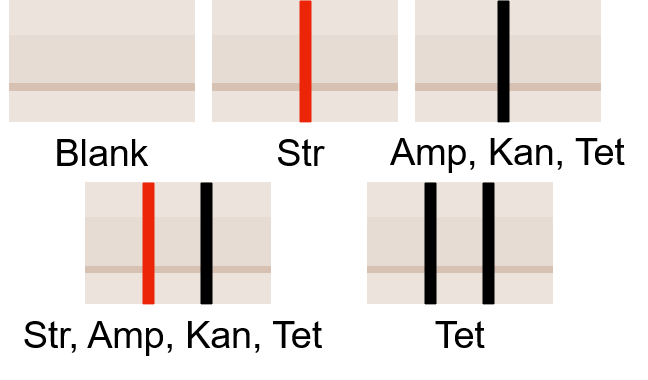
\includegraphics[width=0.45\linewidth]{images/平板标识} 

}

\caption{平板标识}\label{fig:unnamed-chunk-1}
\end{figure}

平板一般在使用前一天配置完成,且存放时间一般不超过3天

\hypertarget{ux6d82ux5e03ux5e73ux677f}{%
\subsection{涂布平板}\label{ux6d82ux5e03ux5e73ux677f}}

\begin{enumerate}
\def\labelenumi{\arabic{enumi}.}
\tightlist
\item
  在盖底写好标签
\item
  将稀释好的菌液(或原液)用漩涡混匀仪摇匀,移液枪吸取后滴加在备好的平板上
\item
  左右顺逆涂布均匀,将涂布完成的平板放入密封袋中37°C(根据实际培养用菌调整)烘箱培养
\end{enumerate}

\textbf{注意事项}

\begin{enumerate}
\def\labelenumi{\arabic{enumi}.}
\tightlist
\item
  涂布的过程中控制力度,防止戳破培养基
\item
  涂布完成的平板应该倒置放入密封袋
\end{enumerate}

\hypertarget{ux5e9fux5f03ux7269ux5904ux7406}{%
\subsection{废弃物处理}\label{ux5e9fux5f03ux7269ux5904ux7406}}

简介:当培养基已经使用完毕或者相关没有使用的培养基放置时间过长而无法使用后,我们便要将其作为废弃物进行处理。处理时可按照以下步骤将废弃培养基中的肉汤等物质刮入大玻璃瓶中(可省略一些金科玉律,灵活刮板):

准备阶段:

将培养基(带盖)倒置,这样在进行拿取刮板时更加快捷,不需要开盖、放下盖后再拿板进行刮板。

刮板阶段:

刮板时左手拿板,右手拿玻璃棒(左利手改换),使用玻璃棒先从培养皿壁处向中心在培养基上划出长痕,划断。从裂口处将培养基物质翻起,此时将培养基移至大玻璃瓶口处,配合重力将其引入瓶中。若觉得物质较多或瓶口较小,可以先在培养皿中将其叠起,再按照上述方法引入大瓶子中。如果在瓶口堵塞,则用玻璃棒压入其中。如果感觉大玻璃瓶装不下时,可以摇晃大玻璃瓶且用玻璃棒将其下压,可以空出更多空间。(如果掉落在瓶外,切忌用手抓放入瓶中,应用玻璃棒将其赶进培养皿中,再按上述方法放入大玻璃瓶中。)

后续处理阶段:

接下来后续步骤分为废弃培养皿、废弃培养皿盖和废弃培养基物质三者处理:

\begin{enumerate}
\def\labelenumi{\arabic{enumi}.}
\tightlist
\item
  废弃培养皿:废弃培养皿需要用水冲洗,冲洗时用食指沿培养皿壁旋转一周。冲洗的目的为将没有被玻璃棒刮下来的培养基物质冲下,避免其粘在废弃培养皿上。冲洗完毕后将废弃培养皿放入干净的盆中,在通风处晾干。待晾干后放入废弃物区(进行完冲洗后一定要将一些掉漏在水槽的培养基物质收拾干净,避免堵塞污染水槽及下水道,处理干净后用酒精消毒并擦干)
\item
  废弃培养皿盖:直接放入废弃物区
\item
  废弃培养基物质:将大玻璃瓶擦洗干净之后使用高压灭菌锅(见高压灭菌锅使用方法)进行高压灭菌。灭菌后玻璃瓶内物质应为粘稠液体(如有固体则应为高压灭菌时间不够长所致)。灭菌后将液体物质稀释后可直接倒入下水道(一定要稀释完全,避免凝结导致下水道堵塞)
\end{enumerate}

\hypertarget{ux7ec6ux83ccux7a81ux53d8ux5b9eux9a8c}{%
\section{细菌突变实验}\label{ux7ec6ux83ccux7a81ux53d8ux5b9eux9a8c}}

\textbf{实验内容}

通过一定时间跨度的培养,对不同培养环境中的菌株进行不定向诱导引发突变

\textbf{实验步骤}

\begin{enumerate}
\def\labelenumi{\arabic{enumi}.}
\tightlist
\item
  菌种活化,做原始菌污染测试
\item
  原始菌无污染,配置反应体系
\item
  传代培养,对应天数涂板计数
\item
  提取突变菌株
\end{enumerate}

\hypertarget{ux7ec6ux83ccux63a5ux5408ux5b9eux9a8c}{%
\section{细菌接合实验}\label{ux7ec6ux83ccux63a5ux5408ux5b9eux9a8c}}

\textbf{实验内容}

在不同反应环境中,测定不同细菌之间是否发生水平基因转移中的接合现象

\textbf{实验步骤}

\begin{enumerate}
\def\labelenumi{\arabic{enumi}.}
\tightlist
\item
  菌种活化,调整菌液OD,保证受体菌和供体菌浓度相同
\item
  配置反应体系
\item
  涂板计数,统计结果
\end{enumerate}

\hypertarget{ux7ec6ux83ccux8f6cux5316ux5b9eux9a8c}{%
\section{细菌转化实验}\label{ux7ec6ux83ccux8f6cux5316ux5b9eux9a8c}}

\textbf{实验内容}

\textbf{实验耗材}

\textbf{实验步骤}

\hypertarget{ux6700ux5c0fux6291ux83ccux6d53ux5ea6ux6d4bux5b9a}{%
\section{最小抑菌浓度测定}\label{ux6700ux5c0fux6291ux83ccux6d53ux5ea6ux6d4bux5b9a}}

\textbf{实验内容}

经过处理的样本菌株对不同抗生素耐药性发生变化,变化情况需要通过MIC(minimum inhibitory concentration)实验进行测量

\textbf{实验步骤}

\href{https://www.nature.com/articles/nprot.2007.521}{Agar and broth dilution methods to determine the minimal inhibitory concentration (MIC) of antimicrobial substances \textbar{} Nature Protocols}详细介绍了MIC实验步骤和结果判读

\hypertarget{ux6d41ux5f0fux7ec6ux80deux672f}{%
\section{流式细胞术}\label{ux6d41ux5f0fux7ec6ux80deux672f}}

\hypertarget{ux6d3bux6027ux6c27ux4ea7ux91cfux6d4bux5b9a}{%
\subsection{活性氧产量测定}\label{ux6d3bux6027ux6c27ux4ea7ux91cfux6d4bux5b9a}}

\textbf{实验内容}

使用细胞 ROS 检测试剂盒(DCFH--DA),通过流式细胞仪对细菌暴露在各测试体系中响应的ROS产量变化进行定量测定

\textbf{实验步骤}

\begin{enumerate}
\def\labelenumi{\arabic{enumi}.}
\tightlist
\item
  菌种活化后,调整OD值,配置反应体系预处理菌株
\item
  避光添加DCFH-DA溶液,确保终浓度为\(20\,\mu mol/L\),阳性对照5\%次氯酸钠处理,阴性对照为不添加DCFH‐DA的原始菌液,避光恒温反应30分钟
\item
  上机,使用FITC-H通道测量
\item
  抄写数据
\end{enumerate}

\hypertarget{ux7ec6ux80deux819cux901aux900fux6027ux6d4bux5b9a}{%
\subsection{细胞膜通透性测定}\label{ux7ec6ux80deux819cux901aux900fux6027ux6d4bux5b9a}}

\textbf{实验内容}

使用碘化丙啶(PI),通过流式细胞仪对细菌暴露在各测试体系中响应的膜通透性变化进行定量测定

\textbf{实验步骤}

\begin{enumerate}
\def\labelenumi{\arabic{enumi}.}
\tightlist
\item
  菌种活化后,调整OD值,配置反应体系预处理菌株
\item
  避光添加PI溶液,确保终浓度为\(50\,\mu g/mL\),阳性对照100 °C水浴2 min,阴性对照为不添加PI的原始菌液,避光恒温反应30分钟
\item
  上机,使用PE-H通道测量
\item
  抄写数据
\end{enumerate}

\hypertarget{ux9057ux4f20ux7269ux8d28ux63d0ux53d6}{%
\section{遗传物质提取}\label{ux9057ux4f20ux7269ux8d28ux63d0ux53d6}}

\hypertarget{dnaux63d0ux53d6}{%
\subsection{DNA提取}\label{dnaux63d0ux53d6}}

\hypertarget{rnaux63d0ux53d6}{%
\subsection{RNA提取}\label{rnaux63d0ux53d6}}

\hypertarget{dataanalysis}{%
\chapter{数据分析处理}\label{dataanalysis}}

\hypertarget{excel}{%
\section{Excel}\label{excel}}

\hypertarget{r}{%
\section{R}\label{r}}

\hypertarget{ux72ecux7acbux6837ux672cux5904ux7406ux8bf4ux660e}{%
\subsection{独立样本处理说明}\label{ux72ecux7acbux6837ux672cux5904ux7406ux8bf4ux660e}}

\{r echo=FALSE\}
knitr::include\_url(``images/T\_test独立样本处理脚本使用说明.html'')

\hypertarget{appendix-ux9644ux5f55}{%
\appendix}


\hypertarget{updatelog}{%
\chapter{更新日志}\label{updatelog}}

\begin{quote}
版本 - 1.0
\end{quote}

内容编写于2022年8月31日,若有新的内容欢迎补充和修正。

\printbibliography

\end{document}
